%% MDPI Computers submission -- generated from the IOS Press draft.
%% Build: pdflatex main && pdflatex main
\documentclass[computers,article,submit,moreauthors]{Definitions/mdpi}

\firstpage{1}
\makeatletter
\setcounter{page}{\@firstpage}
\makeatother
\pubvolume{1}
\issuenum{1}
\articlenumber{0}
\pubyear{2026}
\copyrightyear{2026}
\datereceived{ }
\daterevised{ }
\dateaccepted{ }
\datepublished{ }

% not loaded by the class file
\usepackage{algpseudocode}
\usetikzlibrary{arrows.meta,positioning}
\DeclareFloatingEnvironment[fileext=loa,listname={List of Algorithms},name=Algorithm]{algo}

\renewcommand{\algorithmicrequire}{\textbf{Input:}}
\renewcommand{\algorithmicensure}{\textbf{Output:}}

%=================================================================
\Title{Verifiability-Typed Review Knowledge with Human-Gated Evolution for LLM-Assisted Review of Technical Solution Proposals}

% TODO: replace placeholder author, affiliation and ORCID before submission.
\newcommand{\orcidauthorA}{0000-0000-0000-0000}

\Author{Firstname Lastname $^{1}$\orcidA{}}
\AuthorNames{Firstname Lastname}
\address{%
$^{1}$ \quad Organisation, City, Country; first.author@example.com}
\corres{Correspondence: first.author@example.com}

\abstract{Large language models (LLMs) increasingly pre-screen technical documents before an expert signs off, yet expert review knowledge enters such systems as keyword rules, prompt checklists, or retrieval over past reviews. Each route loses a property that high-stakes review needs: findings must trace to a rule and a document location, decision authority must match how deterministically a requirement can be checked, knowledge must grow from use, and that growth must stay under human control. We call this the \emph{review-knowledge ingestion problem} and study it for the preliminary review of technical solution proposals at a large utility. Knowledge becomes a versioned package of verifiability-typed rules: \emph{hard} rules are owned by deterministic verifiers that produce located evidence, including absence evidence an LLM may never assert; \emph{hybrid} rules let verifiers locate candidate spans and cues while the LLM judges only inside them, enforced by a tool-side evidence gate; \emph{soft} rules only raise items for human judgement. A deterministic policy derives the suggested verdict; only the expert writes the final one. Expert decisions become an audited learned layer that may tune parameters and phrasing but can never promote a rule's tier. Implemented as a plugin of an open-source agent harness (28 rules, no separate backend), the design reaches F1 0.798 against 0.222 for a keyword baseline on a synthetic corpus with planted defects, with no false positive and 85\% verdict agreement ($\kappa=0.76$); 80\% of the remaining misses surface to the expert as open items. Re-expressing the legacy checklist showed that only 10 of 28 rules are deterministically verifiable, and the four blocking rules least of all.}

\keyword{large language models; document review; human-in-the-loop; neuro-symbolic verification; knowledge engineering; evidence grounding}

\begin{document}

\section{Introduction}

Before a change to a large online service platform is built, its \emph{technical solution proposal}---a templated document describing background, architecture, interfaces, data flows, implementation plan and risk---must be reviewed by a small group of senior experts. The review is checklist-driven, the documents are highly templated, the consequences are real (the expert signs the opinion), and the knowledge is both specialised and changing. These properties make preliminary review a natural target for LLM assistance; they also make the usual way of building that assistance fragile.

Our starting point is a failed first attempt. A monolithic prototype built in 2025 encoded 24 expert rules as a few keywords each and delegated the rest to an LLM through long prompts. ``Load test'' appearing anywhere counted as the load test having been planned; negations (``no load test is planned for now''), placeholders (``/'', ``N/A'') and empty sections were invisible; the verdict was whatever the model wrote in a single field, so a blocking finding did not change the outcome; and nothing was persisted, so the hundredth review was no better informed than the first. None of these was a failure of the model. They were failures of \emph{how the review knowledge had been put into the system}.

Three ingestion routes dominate practice. \emph{Keywording} turns a rule into substrings and loses its meaning. \emph{Prompting} turns a rule into instructions and loses auditability: the model has seen the rule, but its judgement cannot be traced to the rule or to a document location. \emph{Fragmenting}---retrieval over past reviews---loses accumulation: knowledge is reassembled at every query and never consolidated. All three treat knowledge as input shown to the model rather than as an asset owned by the system. Two tensions underlie this. The \emph{verifiability tension}: requirements span a spectrum from ``the implementation-plan section exists and is not a placeholder'', which a program can check exactly, to ``the risk analysis is adequate'', which is almost entirely judgement; the less verifiable a requirement, the more it needs a model, and the more verifiable it is, the less a model should be trusted with it, because models make unexplained errors on deterministic questions and cannot locate them~\cite{liu2024lost,huang2024self}. The \emph{growth tension}: knowledge must grow from use---every dismissal is information---but where a human signs the outcome growth cannot be unilateral, and growth in weights or filter thresholds is invisible to those accountable for it.

We make four contributions: (1) we formulate the review-knowledge ingestion problem and derive four design requirements---\emph{auditability}, \emph{authority follows verifiability}, \emph{growth}, \emph{bounded growth}; (2) a \emph{verifiability-typed} rule model in which the type decides who may raise a finding, with absence as a verifier-owned evidence kind and a deterministic verdict policy; (3) \emph{review as feedback}, in which the expert's ordinary decisions are the only source of change to a learned layer that the system may tune but never promote; and (4) a plugin-native implementation evaluated on a corpus with planted defects. We answer one question per property: \textbf{RQ1} can every finding be traced to a rule and a location? \textbf{RQ2} does typed authority outperform untyped authority, and does the type predict expert disagreement? \textbf{RQ3} does the knowledge measurably grow? \textbf{RQ4} is all growth human-attributable and reversible?

\section{Related Work}

\paragraph{Inspection and requirements quality.}
Checklist-based reading has been the backbone of document and code inspection since Fagan~\cite{fagan1976}, and surveys stress that reading technique, not reviewer talent, determines yield~\cite{lait2000}. Verifiability is a defined quality attribute of a requirement~\cite{iso29148,genova2013}, and requirements smells---weak words, placeholders, missing units---are detected with lightweight deterministic analysers precisely because these are cheap, explainable and stable~\cite{femmer2017}. Our verifiers inherit this tradition; the contribution is to use verifiability as a \emph{type} that governs what the model may do.

\paragraph{LLMs for requirements and design review.}
Surveys of LLM use in requirements engineering identify hybrid LLM--tool pipelines and human-in-the-loop control as the main responses to hallucination and inconsistency~\cite{hemmat2025,huang2025hall}, and reviews of LLMs paired with static analysers stress that verification, not generation, is the bottleneck~\cite{dolcetti2025}. Multi-agent validators such as MARV retrieve standards into role prompts and report high recall with over-flagging~\cite{chinnam2025}. ReqPlan-Eval routes requirements to human review on evidence signals, keeps decision authority with the reviewer, and states what its evidence does not establish~\cite{alsawalqah2026}. We share the evidence-first, human-controlled stance but make the knowledge itself an asset with types and a life cycle.

\paragraph{Neuro-symbolic compliance review.}
PolicyGuard compiles organisational policy into typed relational logic rules whose ground atoms are answered by an LLM from retrieved evidence before a symbolic evaluator applies the rule~\cite{malik2026}. It satisfies auditability and partially separates authority, but the separation is \emph{symmetric}---every atom is answered by the LLM---and it has no notion of a requirement the model must not be asked at all, no feedback loop and no bounded evolution. Neuro-symbolic integration in general aims to let symbolic components constrain learned ones~\cite{garcez2023}; our contribution is a specific constraint, that evidence must fall inside verifier-located spans, plus a static type check that rejects packages violating it.

\paragraph{Feedback-driven review and grounding.}
Industrial code review learns from developer reactions: BitsAI-CR prunes rules using an outdated-rate proxy for adoption~\cite{sun2025}, and mining 31{,}073 CodeRabbit review--feedback pairs showed 56.3\% of agentic comments rejected, mainly as false positives or misalignment, and that rejection is predictable~\cite{lin2026}. In all of these, learning happens in the model, a filter or a vendor-operated pruning step; the reviewer cannot see it or roll it back, and the object of review is code rather than a design document. Attributed generation attaches citations to claims~\cite{gao2023}, and models can produce verbatim quotes for most claims yet those quotes substantiate far fewer~\cite{zhang2026cite}. We add two constraints the citation literature does not need: quotes must lie in a span chosen by a verifier, and absence can never be claimed by the model. Self-refinement and reflection let agents improve their own outputs or memory~\cite{madaan2023,shinn2023}, and open-ended self-modifying agents exist~\cite{zhang2025dgm}; we treat ``which layer of the knowledge may the system change on its own'' as a design decision fixed by type. Our protocol is machine teaching in the strict sense, and the dashboard exposes what has been learned per rule.

\section{Materials and Methods}

\subsection{Problem Formulation and Design Requirements}

Let $K$ be a body of review knowledge---rules, phrasing exemplars and past decisions---and $S$ an LLM-based system that, given a document $d$, produces findings and a suggested verdict. The \emph{review-knowledge ingestion problem} is to choose a representation of $K$ and an assignment of decision authority over it such that:
\begin{enumerate}[label=\textbf{(\roman*)},leftmargin=*]
\item \textbf{Auditability.} Every finding traces to an element of $K$ and to a location in $d$, or to an explicit verifier-produced statement that something expected is absent.
\item \textbf{Authority follows verifiability.} Whether $S$ may raise a finding automatically, raise it subject to a check, or only flag it for a human is a function of how deterministically the element of $K$ can be checked against $d$.
\item \textbf{Growth.} $K$ is updated incrementally from the interaction between expert and system, without a separate annotation process.
\item \textbf{Bounded growth.} Every update is attributable to a human decision, constrained by (ii), and reversible.
\end{enumerate}
We use these rather than issue-level accuracy as the primary lens because accuracy against a direct-prompting baseline is overtaken by the next model generation, whereas (i)--(iv) are properties of the organisation, not of the model.

\subsection{Verifiability-Typed Rules}

A rule package is a YAML file validated on load. Each rule has an identifier, a review dimension (capacity, security, interface, channel, data synchronisation, configuration, monitoring, documentation), a severity (blocker, major, minor), a \emph{tier}, the question put to the LLM and the expert, a rationale, a default remediation, an optional applicability precondition, a verifier specification and a status. The package also carries a lexicon---heading aliases, placeholder tokens, negation tokens and keyword families (e.g.\ \emph{loadtest} = load, stress and performance testing in Chinese)---which rules reference by key.

The tier is the type of the knowledge (Table~\ref{tab:tiers}). The criterion is operational: \emph{can a deterministic procedure produce located evidence for or against the requirement, including evidence of absence?} If yes for every aspect, the rule is hard; if a procedure can locate where the requirement would be addressed and flag surface cues (negation, placeholder, unjustified assertion) but the judgement requires reading, it is hybrid; if no procedure can locate relevant text reliably, it is soft.

\begin{table}[H]
\caption{Tier semantics. ``Who may raise a finding'' is enforced in the tools, not in the prompt.}
\label{tab:tiers}
\centering
\small
\begin{tabularx}{\textwidth}{@{}lXXX@{}}
\toprule
Tier & Verifier & Outcomes & Who may raise a finding \\
\midrule
hard & required; every sub-check decisive & pass, fail, not applicable & only the verifier; an LLM attempt is rejected \\
hybrid & required & candidate, pass (structural only), pending, not applicable & structural fail automatic; LLM only inside candidate spans; no candidate $\rightarrow$ pending, never fail \\
soft & forbidden & --- & LLM may register; always pending, never counted \\
\bottomrule
\end{tabularx}
\end{table}

The type is checked statically when the package loads, and a package is rejected as a whole if a rule breaks an invariant: a soft rule with a verifier; a hard or hybrid rule without one; a hard rule whose verifier tree contains a non-decisive check or a pending no-candidate branch; a hybrid rule whose statement check is decisive or whose no-candidate behaviour is fail; a missing lexicon key; or a duplicate identifier. These invariants are the executable form of (ii): a rule whose stated verifiability and whose authority disagree cannot be shipped.

Two consequences follow. First, \emph{absence is verifier-owned}: ``load testing is not mentioned'' cannot be quoted, and an LLM claim of it is unverifiable by construction; only hard verifiers emit absence evidence, a hybrid rule with no candidate becomes pending, and an LLM submission of absence---or a quote beginning with ``not mentioned'', ``missing'' and similar---is rejected. Second, \emph{candidate existence is not satisfaction}: a hybrid statement check never yields pass, and if the LLM registers nothing the checklist says ``reviewed, no issue'' rather than ``pass''.

\subsection{Verifiers and the Evidence Gate}

Documents are Markdown; Word and PDF inputs are converted by a pre-existing office plugin of the host, so the review plugin contains no converter. The parser builds a heading tree with section paths, tables with cell ranges, Mermaid sequence diagrams with participants and messages, and a normalised text layer (NFKC folding, full-width to half-width punctuation, emphasis removal, whitespace collapsing) with an offset map back to the source, so any match is reported as a source range.

Six verifier families and two combinators cover the package. \emph{section} checks that a heading exists, its body exceeds a minimum length and is not a placeholder; \emph{table} locates a table and checks required column groups, placeholder cells and a required row; \emph{statement} finds sentences hitting keyword families, detects negation within a window and assertions without causal justification, and can run in decisive mode for hard rules (16 uses); \emph{quantity} requires a number with a unit near a context family---``expected 500k new users per month'' versus ``a large number of new users''; \emph{mermaid-sequence} requires a Mermaid diagram (an image is a fail, being unverifiable), minimum participants and messages, and specific message families; \emph{cross-ref} requires every ``see Attachment $n$'' to resolve to an entry in the attachment list. Sentences are split at Chinese and Latin terminators and at table-cell boundaries, so a cell is itself a candidate unit; absence evidence carries a zero-length range where the expected content would appear.

The LLM writes findings only through one tool whose implementation runs the gate (Algorithm~\ref{alg:gate}). A finding is confirmed only if every step passes; otherwise it is stored as pending with the full list of reasons, so the agent can repair the quote once and the reasons can be analysed later. Gate decisions are deterministic and recorded per review.

\begin{algo}[H]
\caption{Evidence gate (simplified).}
\label{alg:gate}
\begin{algorithmic}[1]
\Require review, rule id (optional), evidence list
\State resolve rule; if undefined \textbf{then} reason $\leftarrow$ no rule, tier $\leftarrow$ soft
\If{tier $=$ soft} reason $\leftarrow$ soft rule \EndIf
\If{tier $=$ hard} \textbf{raise} hard-rule-verifier-owned \EndIf
\If{evidence empty} reason $\leftarrow$ no evidence \EndIf
\For{all $e$ in evidence}
  \If{kind$(e)=$ absence \textbf{or} quote starts with an absence marker}
    reason $\leftarrow$ absence not allowed \EndIf
  \State $q\leftarrow$ normalise$(e.\text{quote})$; \textbf{if} $|q|<8$ or $|q|>300$ \textbf{then} reason $\leftarrow$ bad length
  \State $h\leftarrow$ locate$(q,d)$ preferring the stated section, then candidate spans, then first hit
  \If{$h=$ none} reason $\leftarrow$ quote not found \Else{} $e.\text{range}\leftarrow h$ \EndIf
  \If{tier $=$ hybrid \textbf{and} $h$ outer to candidates} reason $\leftarrow$ out of candidates \EndIf
\EndFor
\State \Return confirmed \textbf{if} no reason, pending otherwise
\end{algorithmic}
\end{algo}

\subsection{Deterministic Verdict Policy}

The suggested verdict is a function of the confirmed findings, never of anything the model writes:
\begin{small}
\begin{align*}
\text{confirmed} &= \{\,i:\ \text{stat}(i)\in\{\text{conf},\text{acc},\text{rw}\}\ \wedge\ \text{tier}(i)\in\{\text{hard},\text{hyb},\text{exp}\}\,\},\\
m &= |\{i\in\text{confirmed}:\ \text{sev}(i)=\text{minor}\}|,\\
\text{verdict} &=
\begin{cases}
\text{Fail}, & \text{if }\exists i\in\text{confirmed}:\ \text{sev}(i)=\text{blocker};\\
\text{Revise}, & \text{if }\exists i:\ \text{sev}(i)=\text{major}\ \text{ or }\ m\ge\theta;\\
\text{Pass}, & \text{otherwise}.
\end{cases}
\end{align*}
\end{small}
Soft and pending items are listed but never counted. Before review only verifier- and gate-confirmed findings count; after review dismissed findings drop out, accepted and rewritten ones stay, and expert-added findings (tier \emph{expert}) count. The policy is recomputed after every decision and shown as the recommendation when the final verdict is requested. The final verdict is written by a single tool action that requires a named reviewer, so no other code path can write it, and the difference between recommended and final verdict is stored as a measure of rubber-stamping.

\subsection{Review as Feedback: Bounded Evolution}

The review happens in one conversation with a preset of the agent harness---a persona, a skill document and a tool allow-list---that prescribes three phases (Figure~\ref{fig:pipeline}). In \emph{preliminary review} the expert pastes Markdown, gives a path or attaches a Word file; the agent parses it (resuming a re-reviewed proposal by content hash), runs the checks, and for each hybrid candidate first recalls the rule's acceptance statistics, recent dismissal reasons and phrasing exemplars, then judges the candidate snippets only and registers findings with a verbatim quote. The gate decides. The status view renders the suggested verdict with counts, findings ordered by severity with quotation and section, the items needing judgement, and a one-line checklist summary.

\begin{figure}[H]
\centering
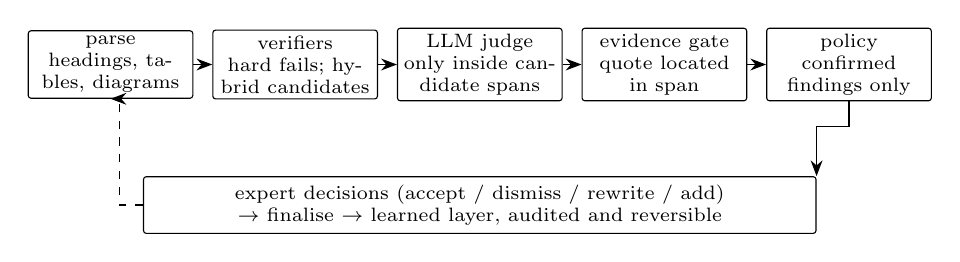
\begin{tikzpicture}[font=\scriptsize,>=Stealth,
  box/.style={draw,rounded corners=1pt,align=center,inner sep=2pt,minimum height=0.72cm,text width=1.95cm},
  arr/.style={->,semithick}, fb/.style={->,semithick,dashed}]
\node[box] (parse) {parse\\headings, tables, diagrams};
\node[box,right=0.24cm of parse] (ver) {verifiers\\hard fails; hybrid candidates};
\node[box,right=0.24cm of ver] (judge) {LLM judge\\only inside candidate spans};
\node[box,right=0.24cm of judge] (gate) {evidence gate\\quote located in span};
\node[box,right=0.24cm of gate] (policy) {policy\\confirmed findings only};
\node[box,below=0.95cm of judge,text width=8.4cm] (fb) {expert decisions (accept / dismiss / rewrite / add) $\rightarrow$ finalise $\rightarrow$ learned layer, audited and reversible};
\draw[arr] (parse)--(ver);
\draw[arr] (ver)--(judge);
\draw[arr] (judge)--(gate);
\draw[arr] (gate)--(policy);
\draw[arr] (policy.south) -- ++(0,-0.32) -| (fb.north east);
\draw[fb] (fb.west) -- ++(-0.3,0) |- (parse.south);
\end{tikzpicture}
\caption{Review pipeline. The verifier decides what may be checked automatically, the gate decides whether the model's evidence is admissible in position, and the policy computes the suggested verdict from confirmed findings only. The dashed path is the only way in which knowledge changes.}
\label{fig:pipeline}
\end{figure}

In \emph{expert review} the agent presents findings in batches of at most five through the harness's structured question tool, each with the quotation and the proposed remediation and with three options: fix as suggested, no change needed, fix but in my words. Free text is normalised by the tool rather than by the model: ``agreed'' becomes accept; ``not an issue'' or ``already covered'' becomes dismiss with the remainder stored as the reason; ``change it to:'' becomes rewrite; ``make it minor'' becomes accept with a per-finding severity override that does not touch the rule; ``you missed'' becomes add, matched to the closest rule if any. ``Accept the rest'' accepts only confirmed findings, and pending items must each be looked at. In \emph{finalisation} the system renders the formal opinion, delivers it as a file and atomically updates the knowledge layer; a later decision reopens the record and requires a new version. The protocol is machine teaching by ordinary work: the expert never labels anything, and every decision the expert must take anyway becomes a typed event.

Knowledge lives in two layers. The \emph{shipped} layer is the rule package; the \emph{learned} layer is a set of records merged over it at read time---per-rule overrides (status, severity, suggestion text and a whitelist of verifier parameters), per-rule statistics, phrasing exemplars, candidate rules from expert-added findings that matched no rule, and draft rules that the agent writes in YAML from a candidate and that become active only when the expert accepts them. Every write appends an audit entry, and an \emph{effective knowledge version} \texttt{pack@ver+ovN} is stamped on every review, where $N$ counts rules with an active override, so a review can be reproduced against the knowledge that produced it.

The boundary is deliberately asymmetric. The system may change parameters within the whitelist, phrasing, severity and status, and may draft new \emph{soft} rules, but it can never raise a rule's tier: a draft claiming to be hybrid or hard must carry a verifier a human has reviewed. Promotion of authority is thus a human act by construction, which is our reading of (iv). Reversal is symmetric: setting a field back to its shipped value deletes the override, so ``changed back'' and ``never changed'' are indistinguishable in the effective version, and a reset removes all overrides of a rule in one audited step while keeping its statistics.

\subsection{Implementation}

We implemented the design as \emph{SolutionReview}, a plugin bundle for an open-source conversational agent harness that already provides the conversation loop, model access, file access, a structured question tool, a delivery tool, a persona/skill mechanism, a JSON-backed storage service, a web server with access control and layout slots. The plugin adds a pure-function engine (parser, verifiers, gate, policy, memory aggregation, opinion renderer; no I/O and no clock), a storage domain with seven tables, nine tools exposed only inside the review preset, three slash commands that query state without the model, an HTTP API under the host's access control, and a dashboard with an overview, a rules page and a sidebar assistant. There is no separate backend, database, embedding index or front-end build; the client is a single 80 kB bundle. Tool contracts are schema-checked with thirteen typed error codes, re-running a check after a decision is refused (it would orphan feedback), and an already reviewed proposal is resumed rather than duplicated.

\section{Results}

\subsection{Setup}

\paragraph{Corpus.}
The released generator (seed 20261029) produced 100 proposals with 253 planted defects over the 23 verifiable rules---98 \emph{absent}, 37 \emph{negated}, 52 \emph{placeholder} and 66 \emph{keyword-present-but-empty}---from phrase pools in which each rule has at least three satisfied and four unsatisfied phrasings, including at least one that avoids the lexicon keywords. Expected verdicts are 30 Pass, 47 Revise and 23 Fail, with 30 proposals shaped on the 15/14/1 verdict distribution of 30 historical expert opinions. The corpus is synthetic because the original proposals could not be released; it measures mechanism correctness and relative baselines, not business-semantic judgement. Every satisfied phrasing passes a self-check: on the 100 proposals no verifier fails and no finding is raised on an unplanted rule (0 violations), so a reported false positive is attributable to the mechanism rather than to the corpus. Building the corpus surfaced one real defect in the shipped package: the attachment-list pattern of the prototype-comparison rule did not capture the attachment number, so a correctly listed prototype attachment was reported missing on every UI-change proposal; the pattern was corrected and the fix is covered by the self-check.

\paragraph{Configurations and metrics.}
We compare B0, which replicates the 2025 prototype (3--5 substrings per rule, no negation detection, no structure, no evidence) but applies the same verdict policy more leniently than the prototype, with the typed design S-full (verifiers, candidates, gate, policy, memory) and with S$-$verifier, where hybrid statements are evaluated over the whole document. The plugin ships no model client; hybrid judgements go through a pluggable judge. We report the deterministic \emph{flag judge}, which raises a finding on a candidate span exactly when the verifier marked it negated, assertion-only or placeholder. It measures the mechanism, not LLM capability; the LLM-judge configurations (direct prompting, gate disabled, model-stated verdict) are left to a companion report rather than approximated. Alignment is at (review, rule) granularity. We report precision, recall, F1 with bootstrap intervals over proposals, severity-weighted recall (weights 3/2/1), verdict accuracy, macro-F1, Cohen's $\kappa$ unweighted and quadratically weighted~\cite{cohen1960,landis1977}, evidence validity (share of model registrations that passed the gate) and pending coverage (share of misses shown to the expert as open items).

\subsection{Typing the Legacy Rule Set}

Re-expressing the 24 legacy rules under the typing criterion produced 6 hard, 13 hybrid and 5 soft rules; with four template-derived structural rules (quantified business volume, change-list table, mandatory sections, attachment consistency) the shipped package has 10 hard, 13 hybrid and 5 soft rules. Fewer than half of the rules the prototype implemented as keyword checks are deterministically verifiable, and thirteen require reading a located passage---exactly the case in which keyword presence is uninformative. Severity and verifiability are also inversely related: all four \emph{blocker} rules (rate limiting, encryption and signing, a closed authorisation chain, data exposure) are hybrid, and all ten hard rules are major or minor. The most consequential requirements are the ones a program can locate but not decide, which is where the gate and the expert's attention are concentrated. Seven rules carry applicability preconditions, which turns ``not applicable'' into an explicit checklist state rather than a silent pass; the lexicon has 23 keyword families, 11 heading groups, 12 placeholder tokens and 11 negation tokens.

\subsection{Results on the Synthetic Corpus}

Table~\ref{tab:results} reports the results; three repetitions of each configuration produced byte-identical metrics, so the intervals are bootstrap intervals over proposals, not repetition variance.

\begin{table}[H]
\caption{Issue-level and verdict-level results on the synthetic corpus (100 proposals, 253 planted defects; deterministic configurations; 95\% bootstrap CIs by proposal; S-full and S$-$verifier are identical under the deterministic judge).}
\label{tab:results}
\centering
\footnotesize
\setlength{\tabcolsep}{4pt}
\begin{tabularx}{\textwidth}{@{}l*{2}{>{\centering\arraybackslash}X}>{\centering\arraybackslash}p{3.6cm}*{5}{>{\centering\arraybackslash}X}@{}}
\toprule
Configuration & P & R & F1 [95\% CI] & $R_w$ & Verdict acc. & macro-F1 & $\kappa$ & $\kappa_w$ \\
\midrule
B0 keyword & 0.275 & 0.186 & 0.222 [0.176, 0.267] & 0.162 & 28.0\% & 0.275 & $-0.043$ & $-0.059$ \\
S-full & \textbf{1.000} & \textbf{0.664} & \textbf{0.798} [0.762, 0.836] & \textbf{0.649} & \textbf{85.0\%} & \textbf{0.832} & \textbf{0.763} & \textbf{0.739} \\
S$-$verifier & 1.000 & 0.664 & 0.798 [0.762, 0.836] & 0.649 & 85.0\% & 0.832 & 0.763 & 0.739 \\
\bottomrule
\end{tabularx}
\end{table}

\paragraph{Typing versus keywording (RQ2).}
B0 produced 47 true, 124 false and 206 missed findings; S-full produced 168 true findings, no false finding and 85 misses, a gain of $\Delta$F1 $=+0.564$ (paired Wilcoxon signed-rank over per-proposal F1, $p<0.001$; McNemar on verdict correctness $b/c=64/7$, $p<0.001$; both survive Holm correction). B0's errors have the shape the typing predicts: keyword presence is uninformative on negated, placeholder and hollow phrasings (precision 0.00 on 13 of the 23 rules), while keyword absence fires on satisfied phrasings that avoid the lexicon (recall 0.13 on the sequence-diagram rule, 0.29 on the load-test rule). Its verdict agreement is at chance ($\kappa=-0.04$; 17 of 30 Pass proposals rated Fail), reproducing the 2025 failure in which a declared-but-unverifiable checklist drove the verdict.

\paragraph{Where the remaining misses are.}
All 85 misses are either planned pending states or a documented limit of decisive verifiers; none is a silent pass on a located defect. Sixty-eight are hybrid defects reported as \emph{pending}---27 absent and 30 hollow phrasings the flag judge cannot decide, plus 11 negated or placeholder spans rejected by the gate---so 80\% of all misses are shown to the expert as open items rather than hidden. The remaining 17 are hard rules decisive on keyword presence (load-test statement 7, channel identifier 5, change-list table 5) that miss placeholder or hollow phrasings, the documented trade-off for making these rules fully automatic. By planted kind, the mechanism alone located 71 of 98 absent, 31 of 37 negated, 42 of 52 placeholder and 24 of 66 hollow defects; the ordering absent $>$ negated $>$ placeholder $>$ hollow is the ordering of what structure alone can decide, and the hollow kind is exactly the case that needs an LLM judge.

\paragraph{Evidence gate.}
The deterministic judge submitted 53 hybrid findings; 42 passed and 11 (20.8\%, in 10 proposals) were rejected as too short, because negated or placeholder sentences fall below the eight-character quote floor. The rejected findings were downgraded to pending rather than discarded---they are exactly 6 negated and 5 placeholder pending cases---so the gate cost 11 located true findings (recall $-0.043$) and no false one, and each stays visible to the expert. The result identifies the quote floor, chosen to stop one- or two-word ``evidence'', as a parameter to revisit for whole-sentence placeholder spans; no absence, not-found or out-of-candidates rejection occurred, as expected for a judge that quotes the verifier's own span.

\paragraph{Span scoping and verdict policy.}
S$-$verifier is identical to S-full under the deterministic judge ($\Delta$F1 $=0$, $b/c=0/0$): widening the search region added candidate spans but none carried a cue, and the judge never cites outside a region, so the contribution of span scoping is a property of an LLM judge and is measured there. S-full's suggested verdict agreed with the planted verdict in 85 of 100 proposals ($\kappa=0.76$; confusion over Pass/Revise/Fail $[[30,0,0],[6,41,0],[4,5,14]]$). All 15 disagreements are under-calls caused by pending hybrid findings---nine Fail proposals whose blocker defect was hybrid, six Revise proposals whose major defects were hybrid---and there is no over-call, consistent with a policy that counts only confirmed findings.

\subsection{Threats to Validity}

\emph{Construct.} Synthetic ground truth is produced by the same policy function the system uses, so the synthetic verdict comparison tests policy consistency rather than correctness; correctness must be assessed against expert decisions, which we do not have and therefore do not claim. Online labels would treat expert acceptance as truth; experts may rubber-stamp, which is why we would report the share of changed findings, rewrites, additions and dismissals. \emph{External.} One organisation, one template, one rule package in Chinese; the package is data and the engine is template-agnostic, but a second package has not been demonstrated, and hybrid judgements depend on one model family at temperature zero. The historical proposals could not be released and the historical opinions are used only as a distribution. \emph{Reliability.} The engine is deterministic and the gate is recorded, so the mechanism part is reproducible from the released corpus; the LLM part is reproducible only up to provider drift.

\section{Discussion}

\paragraph{Answers to the research questions.}
RQ1 is answered by construction plus exceptions: every finding that reaches the opinion carries a rule and either a located quotation or a verifier-produced absence statement, and the measured quantity is how often the model's first attempt fails the gate and why (79.2\% validity here). RQ2 is answered for its mechanism half: typing, span scoping and the gate raise precision from 0.275 to 1.000 while four fifths of the recall cost is surfaced as pending work rather than lost. Its second half---does the type predict expert disagreement?---needs per-tier dismissal statistics from deployment, which we do not yet have. RQ3 and RQ4 concern the learned layer and are not measured here: knowledge increments per review, the effective-version trajectory, a sliding-window acceptance rate, audit coverage and a degradation-and-reset simulation are the instruments we would report once reviews accumulate. We state this instead of substituting a proxy for growth.

\paragraph{Symmetric versus asymmetric authority.}
PolicyGuard and our design agree that the LLM should not decide compliance and that a symbolic layer should~\cite{malik2026}. They differ on whether the LLM should be asked at all. In PolicyGuard every ground atom is an LLM question whose answer flows into symbolic evaluation, so the model's reliability on each atom is an empirical matter addressed by validation and repair. In our design the type says in advance which questions the model may be asked and on which spans, so a verifier bug and a model error have different signatures---a dismissed hard finding versus a gate rejection or a dismissed hybrid finding---which is what makes per-tier statistics interpretable and the dismissal warning actionable.

\paragraph{Where the learning lives.}
BitsAI-CR prunes rules by an adoption proxy~\cite{sun2025} and CodeRabbit's rejection patterns are learnable by a classifier~\cite{lin2026}; both place learning where the reviewer cannot see it. Our learned layer is human-readable, per rule, versioned and reversible, at the price of being coarser: we adjust parameters within a whitelist, phrasing, severity and status, and we create candidate rules, but we do not learn a filter. We consider this the right trade where the reviewer signs the outcome, because the question the reviewer can answer when a rule starts to misfire is what changed, who changed it and how to undo it. Agent research increasingly studies systems that modify their own tools, prompts or code~\cite{madaan2023,shinn2023,zhang2025dgm}; in an organisational review setting the relevant question is not whether self-modification is possible but where its boundary lies. Our boundary is drawn by type and enforced by static checks and a single write path, not by instructions to the model.

\section{Conclusion}

Putting expert review knowledge into an LLM system is a design problem with its own requirements, not a prompt-engineering detail. We named the problem, stated four properties a solution should have, and showed a design that meets them by typing rules by verifiability, letting the type decide who may raise a finding, gating the model's evidence by position, computing verdicts deterministically, and turning the expert's ordinary decisions into a versioned, auditable, human-gated knowledge layer---all as plugins on an existing agent harness. Typing the legacy checklist already explained the failure of the keyword approach: most of the knowledge was not keyword-verifiable, and the most consequential rules least of all. On a corpus with planted defects the design removes every false positive of the keyword baseline while keeping four fifths of its remaining misses visible to the expert, and its suggested verdicts agree with the planted ones well beyond chance. The plugin, rule package, corpus and evaluation scripts are released for reuse.


\authorcontributions{Conceptualization, X.X.; methodology, X.X.; software, X.X.; validation, X.X.; formal analysis, X.X.; investigation, X.X.; writing---original draft preparation, X.X.; writing---review and editing, X.X.; visualization, X.X. All authors have read and agreed to the published version of the manuscript.} %% TODO: initials

\funding{This research received no external funding.} %% TODO: confirm or add grant number

\institutionalreview{Not applicable.}

\informedconsent{Not applicable.}

\dataavailability{The rule package, synthetic corpus, evaluation scripts and the plugin implementation are available from the authors on request and will be released with the accepted version.} %% TODO: repository DOI

\acknowledgments{The authors thank the reviewing experts of the case organisation.}

\conflictsofinterest{The authors declare no conflicts of interest.}

\reftitle{References}

\isAPAandChicago{}{%
\begin{thebibliography}{999}

\bibitem[Huang et al.(2024)]{huang2024self}
Huang, J.; Chen, X.; Mishra, S.; Zheng, H.S.; Yu, A.W.; Song, X.; et al. Large Language Models Cannot Self-Correct Reasoning Yet. In Proceedings of the Twelfth International Conference on Learning Representations (ICLR 2024), Vienna, Austria, 2024.

\bibitem[Liu et al.(2024)]{liu2024lost}
Liu, N.F.; Lin, K.; Hewitt, J.; Paranjape, A.; Bevilacqua, M.; Petroni, F.; et al. Lost in the Middle: How Language Models Use Long Contexts. {\em Trans. Assoc. Comput. Linguist.} {\bf 2024}, {\em 12}, 157--173. https://doi.org/10.1162/tacl\_a\_00638

\bibitem[Fagan(1976)]{fagan1976}
Fagan, M.E. Design and Code Inspections to Reduce Errors in Program Development. {\em IBM Syst. J.} {\bf 1976}, {\em 15}, 182--211. https://doi.org/10.1147/sj.153.0182

\bibitem[Laitenberger and DeBaud(2000)]{lait2000}
Laitenberger, O.; DeBaud, J.M. An Encompassing Life Cycle Centric Survey of Software Inspection. {\em J. Syst. Softw.} {\bf 2000}, {\em 50}, 5--31. https://doi.org/10.1016/S0164-1212(99)00073-4

\bibitem[ISO/IEC/IEEE(2018)]{iso29148}
ISO/IEC/IEEE. {\em ISO/IEC/IEEE 29148:2018 Systems and Software Engineering---Life Cycle Processes---Requirements Engineering}; International Organization for Standardization: Geneva, Switzerland, 2018.

\bibitem[G\'enova et al.(2013)]{genova2013}
G\'enova, G.; Fuentes, J.M.; Llorens, J.; Hurtado, O.; Moreno, V. A Framework to Measure and Improve the Quality of Textual Requirements. {\em Requir. Eng.} {\bf 2013}, {\em 18}, 25--41. https://doi.org/10.1007/s00766-011-0134-z

\bibitem[Femmer et al.(2017)]{femmer2017}
Femmer, H.; M\'endez Fern\'andez, D.; Wagner, S.; Eder, S. Rapid Quality Assurance with Requirements Smells. {\em J. Syst. Softw.} {\bf 2017}, {\em 123}, 190--213. https://doi.org/10.1016/j.jss.2016.02.047

\bibitem[Hemmat et al.(2025)]{hemmat2025}
Hemmat, A.; Sharbaf, M.; Kolahdouz-Rahimi, S.; Lano, K.; Yassipour Tehrani, S. Research Directions for Using LLM in Software Requirement Engineering: A Systematic Review. {\em Front. Comput. Sci.} {\bf 2025}, {\em 7}, 1519437. https://doi.org/10.3389/fcomp.2025.1519437

\bibitem[Huang et al.(2025)]{huang2025hall}
Huang, L.; Yu, W.; Ma, W.; Zhong, W.; Feng, Z.; Wang, H.; et al. A Survey on Hallucination in Large Language Models: Principles, Taxonomy, Challenges, and Open Questions. {\em ACM Trans. Inf. Syst.} {\bf 2025}, {\em 43}, 42. https://doi.org/10.1145/3703155

\bibitem[Dolcetti and Iotti(2025)]{dolcetti2025}
Dolcetti, G.; Iotti, E. A Dual Perspective Review on Large Language Models and Code Verification. {\em Front. Comput. Sci.} {\bf 2025}, {\em 7}, 1655469. https://doi.org/10.3389/fcomp.2025.1655469

\bibitem[Chinnam(2025)]{chinnam2025}
Chinnam, H. MARV: A Multi-Agent Approach for Validation of Software Requirements Specifications. Master's Thesis, Tampere University, Tampere, Finland, 2025. Available online: https://urn.fi/URN:NBN:fi:tuni-202507297873 (accessed on 30 October 2026).

\bibitem[Alsawalqah et al.(2026)]{alsawalqah2026}
Alsawalqah, H.; Abadleh, A.; Ibrahim, S.; Alqaralleh, B.A.Y.; Aoun, C.; Zreikat, A.I. Evidence-Aware Human-in-the-Loop LLM Review for Requirements-to-Planning Decisions. {\em Computers} {\bf 2026}, {\em 15}, 608. https://doi.org/10.3390/computers15090608

\bibitem[Malik et al.(2026)]{malik2026}
Malik, S.; Singh, A.; Azad, A.P. PolicyGuard: From Organizational Policies to Neuro-Symbolic Compliance Review Engines. \emph{arXiv} {\bf 2026}, arXiv:2606.32004.

\bibitem[Garcez and Lamb(2023)]{garcez2023}
Garcez, A.d'A.; Lamb, L.C. Neurosymbolic AI: The 3rd Wave. {\em Artif. Intell. Rev.} {\bf 2023}, {\em 56}, 12387--12406. https://doi.org/10.1007/s10462-023-10448-w

\bibitem[Sun et al.(2025)]{sun2025}
Sun, T.; Xu, J.; Li, Y.; Yan, Z.; Zhang, G.; Xie, L.; et al. BitsAI-CR: Automated Code Review via LLM in Practice. In Proceedings of the Companion Proceedings of the 33rd ACM International Conference on the Foundations of Software Engineering (FSE Companion '25), Trondheim, Norway, 2025. https://doi.org/10.1145/3696630.3728552

\bibitem[Lin et al.(2026)]{lin2026}
Lin, H.Y.; Liang, M.; Tantithamthavorn, K.; Thongtanunam, P. Is Agentic Code Review Helpful? Mining Developers' Feedback to CodeRabbit Reviews in the Wild. \emph{arXiv} {\bf 2026}, arXiv:2607.03316.

\bibitem[Gao et al.(2023)]{gao2023}
Gao, T.; Yen, H.; Yu, J.; Chen, D. Enabling Large Language Models to Generate Text with Citations. In Proceedings of the 2023 Conference on Empirical Methods in Natural Language Processing (EMNLP 2023), Singapore, 2023; pp. 6465--6488. https://doi.org/10.18653/v1/2023.emnlp-main.398

\bibitem[Zhang et al.(2026)]{zhang2026cite}
Zhang, J.; Chen, Y.; Commodore-Mensah, Y.; Oberst, M. Verifiable by Construction: Claim-Level Evaluation of Verbatim Citation in Clinical Question Answering. \emph{arXiv} {\bf 2026}, arXiv:2609.15964.

\bibitem[Madaan et al.(2023)]{madaan2023}
Madaan, A.; Tandon, N.; Gupta, P.; Hallinan, S.; Gao, L.; Wiegreffe, S.; et al. Self-Refine: Iterative Refinement with Self-Feedback. In Proceedings of the Advances in Neural Information Processing Systems 36 (NeurIPS 2023), New Orleans, LA, USA, 2023.

\bibitem[Shinn et al.(2023)]{shinn2023}
Shinn, N.; Cassano, F.; Gopinath, A.; Narasimhan, K.; Yao, S. Reflexion: Language Agents with Verbal Reinforcement Learning. In Proceedings of the Advances in Neural Information Processing Systems 36 (NeurIPS 2023), New Orleans, LA, USA, 2023.

\bibitem[Zhang et al.(2025)]{zhang2025dgm}
Zhang, J.; Hu, S.; Lu, C.; Lange, R.; Clune, J. Darwin G\"odel Machine: Open-Ended Evolution of Self-Improving Agents. \emph{arXiv} {\bf 2025}, arXiv:2505.22954.

\bibitem[Cohen(1960)]{cohen1960}
Cohen, J. A Coefficient of Agreement for Nominal Scales. {\em Educ. Psychol. Meas.} {\bf 1960}, {\em 20}, 37--46. https://doi.org/10.1177/001316446002000104

\bibitem[Landis and Koch(1977)]{landis1977}
Landis, J.R.; Koch, G.G. The Measurement of Observer Agreement for Categorical Data. {\em Biometrics} {\bf 1977}, {\em 33}, 159--174. https://doi.org/10.2307/2529310

\end{thebibliography}
}

\end{document}
